\section{Shading}

Shading is a way of giving the perception of depth in 3D illustrations.
This is achieved by depicting levels of darkness with respect to a given
light source. This section will attempt to describe to kinds of shading used
in computer graphics, flat and Phong shading. Each section will consist of a
short description of the overall theory behind the shading method followed by a
quick mention of our implementation.

\subsection{Que?}

\subsection{Flat shading}

\subsection{Phong shading}
Flat shading is a little brutal, especially with respect to specularity. If a
surface has large specular areas they will either be ignored, or define the
intensity of the entire surface. Phong illumination corrects this problem.

\begin{figure}[hbt]
	\centering
	\scalebox{0.5}
	{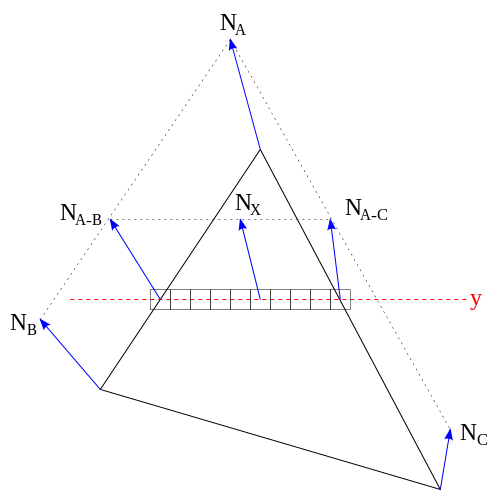
\includegraphics{pics/phongInterpol.png}}
	\caption{Normal interpolation in Phong shading}
	\label{fig:phongInterpo}
\ref{fig:phongInterpo}
\end{figure}

By interpolating the vertex normals across the polygon surface (figure
\ref{fig:phongInterpo}), Phong shading finds a smoothly shifting normal for each
pixel. This normal is then used in the illumination/reflection model, to find
the final intensity weight for that pixel. This will give a much more realistic
result that flat shading, at the expense of interpolating normals and applying
the lighting model for each surface pixel. Figure \ref{fig:fVsP} illustrates
both the improved colour realism (the sphere actually looks spherical), and the
difference in specularity, being completely invisible in the example using flat
shading.

\begin{figure}[htb]
	\centering
	\scalebox{0.7}
	{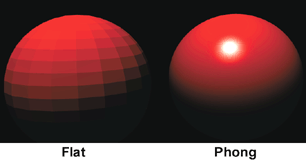
\includegraphics{pics/flatVsPhong.png}}
	\caption{flat vs Phong shading}
	\label{fig:fVsP}
\ref{fig:phongInterpo}
\end{figure}

